\documentclass[journal,final,a4paper,twoside]{PS}

%%% Dieser Block ist dem Betreuer des Projektseminars vorbehalten
\usepackage{PS}             % Alle Definitionen �ber den Seitenstil (auf keinen Fall editieren!!)
\usepackage[T1]{fontenc}
\usepackage[utf8]{inputenc}

\def\lehrveranstaltung{PROJEKTSEMINAR ROBOTIK UND COMPUTATIONAL INTELLIGENCE}
\def\ausgabe{Vol.17,~SS~2017}
\setcounter{page}{1}        % Hier die Seitennummer der Startseite f�r Gesamtdokument festlegen

%%% Ab hier k�nnen Eintr�ge von den Teilnehmern des Projektseminars gemacht werden
%%% Wenn neben den LaTeX-Paketen aus der Datei PS.sty noch weitere gebraucht werden,
%%% so ist dies dringend mit dem Betreuer abzukl�ren!

\begin{document}
\newcommand{\euertitel}{Dynamic Distortion Calibration}   % Titel hier eintragen!
\newcommand{\betreuer}{M. Sc. Raul Acu\~na }  % Betreuerdaten hier eintragen (mit einem Leerzeichen am Ende)!


\headsep 40pt
\title{\euertitel}
% Autorennamen in der Form "Vorname Nachname" angeben, alphabetisch nach Nachname sortieren,
% nach dem letzen Autor kein Komma setzen, sondern mit \thanks abschlie�en
\author{Ahmed Ashraf,
        Nils Hamacher,
        Linghan Qian,
	Vivica Wirth
\thanks{This paper was supported by \betreuer.}}

\maketitle


\begin{Zusammenfassung}
Kameras als Sensoren werden in immer mehr Applikationem im allt\"aglichen Leben wie zum Beispiel in Smartphones, oder um unser Haus mit Hilfe von Smart-Home-Systemen zu \"uberwachen, verwendet. In Fabriken hingegen werden noch viel mehr Kameras zur \"Uberwachung von verschiedensten Prozessen wegen ihrer universellen Anwendung, niedrigen Kosten und dem Potenzial der erhaltenen Daten verwendet. Au\ss{}erdem w\"achst ihre Rolle im Automobilbereich. Jedoch ist jede Kameralinse aufgrund von nicht exakt gleichm\"a\ss{}igen Fertigungstechniken mehr oder weniger gekr\"ummt. Die meisten Kameras zeigen eine radiale Verzerrung, da die Linsen in der Regel eine konvexe Kr\"ummung aufweisen. Diese ist nicht immer gleichm\"a\ss{}ig konvex oder hat Einschl\"usse, die die Verzerrung zu einem sehr nichtlinearen Verhalten ver\"andert. Das macht die Kalibrierung des Kameraobjektivs zu einem wesentlichen Aspekt der Computer Vision, da eine hohe Genauigkeit ihrer Bilder erforderlich ist. Die meisten Kamerakalibrierungen erfordern menschliche Interaktionen wie die Kalibrierung mit einem Schachbrettmuster. In dieser Ausarbeitung wird eine L\"osung f\"ur die Kamera-Kalibrierung vorgestellt, die auf einem planaren Display wie g\"angigen Computermonitoren arbeitet und nicht auf menschliche Interaktion st\"utzt. Dabei wird eine Karte zwischen den Bildschirmpixeln und den projezierten Karmerabildpixeln bestimmt. Wir pr\"asentieren verschiedene Wege, die wir mit ihren Vor- und Nachteilen in Genauigkeit und Laufzeit ausprobiert haben.
\end{Zusammenfassung}
\vspace{6pt}

\begin{abstract}
Cameras as a sensor application are widely used in our daily life like in smartphones or to surveille our home via smart home installation. But even more cameras monitor many processes in factories because of their universal application, low cost and the potential of the obtained data. Also it influence in the automotive branche is rising. However, every camera lens is more or less distorted due to imperfect manufacturing techniques. Most cameras show radial distortion due to the fact that most lenses have convex curvature. These aren't always perfectly convex or got inclusions which do alter the distortion to a very non-linear behavior. That makes calibration of the camera lens an essential aspect of computer vision, since a high accuracy of their images is required. Most camera calibrations require human interactions like the calibration with a checkerboard. In this paper a solution to camera calibration is shown that works on a 2D planar display like common used computer monitors and doesn't rely on human interaction. Therefore a mapping between the screen pixel coordinate system and the image pixel coordinate system is determined. We present different ways we tried with their pros and cons in accuracy and runtime.
\end{abstract}

\section{Introduction}

\PARstart{C}{ameras} are used in more and more situations. Application areas are monitoring technologies, toys, smartphones and increasingly in vehicles for example. However all camera lenses are somewhat different from each other. The curvature of a lens is never perfect, and inclusions may occur which also alter the curvature of the incident light. This leads to distortion that has to be calibrated. State of the art approaches like the checkerboard calibration only base their models on a few interest points. This method for calibration is to position a checkerboard in different poses in front of the camera and detect the intersections of the black and white squares. The more pictures are done the higher is accuracy of the result what increases the human interaction and the time invested. We present this and other methods in Chapter \ref{sec:related}. 
Our aim was to develop a program, which automatically creates a dense model of the lens distortion. This dense model is based on information of the correspondencies of pixels on a screen and the pixels in a captured image. Once the mapping between the screen and the image corresponding pixels is done, we can undistort the image simply by moving the pixels of the actual image we take. In order to reach the desired accuracy we need to set some pre-conditions for the environment in which this takes place. These conditions are darkness, in order to avoid reflections of the camera on the screen, and the camera being perpendicular to the screen. We will present the fundamental principles of several different ideas, which all result in a mapping. To compare them we give a short insight to their runtimes. This article is structured as follows: First follows the related work in \ref{sec:related} then in Chapter \ref{sec:maths} the theoretical  foundations are outlined. Chapter \ref{sec:mapping} includes the idea and realization of the project. In Chapter \ref{sec:results} is the conclusion.


\subsection{Related Work}
\label{sec:related}
Several approaches has been proposed in order to calibrate a camera, they can roughly be classified into two categories [1]: photogrammetric calibration and self-calibration.
Photogrammetric calibration is based on a spatial object with its 3D shape known which is placed in the view of camera. The commonly used object is planar object point array, so called checkerboard pattern [1], or a 3D cube with determined pattern on it. This method is restricted because errors will occur while printing and manually measuring the pattern or also if the pattern isn't always available.\\
In self-calibration [3] a reference object is not required, instead it requires the correspondence between points of the scene and the projection. Duane C B. [5] proposed a nonmetric method, based on the fact that the projection of a straight line from the world space should also be a straight line on the image. Swaminathan R and Nayar S K. [6] extended this method by reducing noise and using polycamera. However, this method still relies on calculating parameters, which is not accurate because the model is simplified. 
Sagawa R  proposed a way using structured light to determine the correspondence and creates directly a dense map so that the error generated by parameter fitting is reduced. 
The system proposed is based on [4] since they are both based on detecting the correspondence of lines and get the map non-parametrically. \cite{Faugeras:1992}

\section{Mathematical Backround}
\label{sec:maths}

\section{Mapping of correspondencing pixels}
\label{sec:mapping}
Our aim was to create a map of corresponding pixels of the screen to the camera image. For that we followed different approaches which we evaluate by accuracy and especially by runtime in Chapter \ref{sec:runtime}. 

\subsection{Pixelwise approaches}
\subsubsection{every Pixel}
\subsubsection{spiral}
\subsubsection{by lines}
\subsection{simple linedetection for x and y matching}
We set the backround of the screen to black. Then we draw a white rectangle with height of the screenheight and an increasing width. At the border of the white rectangle to the black backround the \emph{Canny}-operator detects the points the border as a line. We match to every image pixel that belongs to that line the x coordinate to which it should belong. In figure \ref{fig:blockOverTime} we show how the rectangle is getting wide.
\\

\begin{figure}[h]
\begin{center}
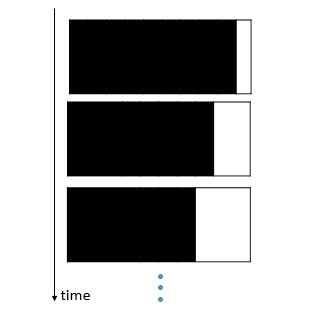
\includegraphics[scale=0.8]{./pics/blockOverTime.jpg}
\caption{Rectangle over time}
\label{fig:blockOverTime}
\end{center}
\end{figure}

\subsection{runtimes of the approaches}
\label{sec:runtime}
\subsubsection{pixelwise}
\label{sec:pixelwise}
Each frame makes one call to the draw function. Given that we need $7$ calls of the draw function to fully draw, capture, and process one image, we can, with a frame rate of $21$ frames per second (FPS), achieve turnover rate of $3$ images per second. This allows us to make an estimation of the runtime of each approach we tested out or considered for the lens calibration. For the following estimates we're assuming a screen of the dimensions $1290 x 1080$ pixels and a field of view (FOV) of roughly $670 x 395$ pixels for the camera. The FOV has been experimentally determined for a distance of 16 cm from the screen. From the results the aperture angle can be calculated, it yields roughly $68.45^{\circ}$, the camera’s specifications state an aperture angle of $68.50 ^{\circ}$ . So these results should be a good estimate of the true FOV. Furthermore the assumption is made that each pixel can be detected on its own, instead of needing larger patches to be detectable by the camera.
The following variables will be use: $h_{FOV}$ as the height of the FOV, $w_{FOV}$ as the width of the FOV, $w_s$ as the width of the screen, and $h_s$ as the height of the screen.
1. Singular pixel detection
With a naive approach each patch of minimal detectable size on the screen has to be turned on separately. This means screen width times screen height necessary images. In our set up $921,600$ images would be needed, yielding a runtime of $307,200$ seconds, or $3$ days $13$ hours $20$ minutes.
It can be sped up however. By lighting up single pixels in a spiral pattern around an estimation of the middle point, the amount of images can be reduced to the amount of pixels within the camera’s FOV runtime to roughly $88,572$ seconds, or $1$ day $1$ hour $30$ minutes.
The center point estimation has been left out, as it is comparably negligible.\\
	
\subsubsection{Line-based detection} 
\label{sec:linebased}
The first idea for a line-based detection was to first detect the borders and store how the border pixels of the image map to the screen. The idea was to first detect a pixel on the border via binary search and then move this pixel to new positions to check whether these are seen. We need to check at least four surrounding pixels for visibility. This means $4 * (2 * h_{FOV} + 2 * w_{FOV})$, in our setup that leads to $8,520$ images. To process these images, we need $2,840$ seconds, or $47$ minutes $20$ seconds. After discovering the border only two images need to be created and processed. However, since the discovery of the border would take still too long, we rejected this method as well.
The next method is a segmentation of the screen. By segmenting the screen sequentially in a black and a white part, we can detect a single edge in the image. The white part starts out as the entire screen and gradually decreases in width, pixel by pixel. After that is done, the white part is again stretched out over the entire screen and then decreases in height. At each image we know exactly at which position the screen shows the edge. From this we can calculate where the edge pixels from the image should have appeared.
When doing this naively and simply going over the entire screen width and height, this method needs to process $2,370$ images. It would take $790$ seconds, or $13$ minutes $10$ seconds. This is already immensely faster. It can still be sped up, however.
Instead of going over the entire screen, we first estimate the center point again. This time we additionally store which was the outermost pixel, which was visible during the estimation, for each border. From there we add the spacing, that was used, plus a small margin to be on the safe side. The margin was chosen to be 5 pixels wide. In this method the runtime for the center point estimation is relevant. While the runtime for the center point estimation increases with smaller spacing, the runtime for the line-based detection decreases. This means a runtime-optimal spacing can be calculated.
Let s be the spacing between the positions of the pixels to be lit, and m the margin. Then the runtime of the center estimation, as a function of spacing s, is:
\begin{align}
rt_c (s) = \frac{w_s\cdot h_s}{ s^2} = 1393200 / s^2.
\end{align}
For the runtime of the line-based detection after that, follows:
\begin{align}
rt_d (s) = 4s + 4\cdot m + w_{FOV} + h_{FOV} = 4s + 1085
\end{align}
From there the overall runtime can be calculated as:
\begin{align}
rt(s) = \frac{1393200}{s^2} + 4s +1085.
\end{align}
This functions minimum is at roughly s = 89. For this spacing we need then $1,617$ images, leading to a runtime of $539$ seconds, or nearly $9$ minutes. Of these roughly $59$ seconds are center point estimation.



\section{results}
\label{sec:results}
\subsection{accuracy}
\subsection{comparation and valuation}


\newpage

\begin{thebibliography}{1}
\bibitem{Faugeras:1992}
O.~Faugeras, Q.T.~Luong and S.~Maybank, \emph{{Camera self-calibration: Theory and experiments}, {pages: 321--334} , {Computer Vision---ECCV'92}}, 1992

\end{thebibliography}

\begin{biography}
[{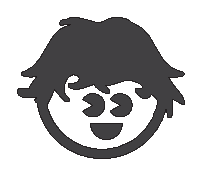
\includegraphics[width=1in,height=1.25in,clip,keepaspectratio]{./pics/ComicKopf.eps}}] % hier ein Foto einbinden
{Autor A}
Biographie Autor A.
\end{biography}
\begin{biography}
[{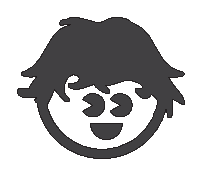
\includegraphics[width=1in,height=1.25in,clip,keepaspectratio]{./pics/ComicKopf.eps}}] % hier ein Foto einbinden
{Autor B}
Biographie Autor B.
\end{biography}
\begin{biography}
[{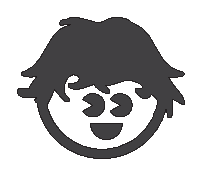
\includegraphics[width=1in,height=1.25in,clip,keepaspectratio]{./pics/ComicKopf.eps}}] % hier ein Foto einbinden
{Autor C}
Biographie Autor C.

\end{biography}

\begin{biography}
[{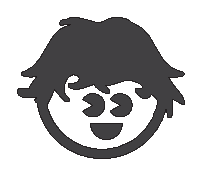
\includegraphics[width=1in,height=1.25in,clip,keepaspectratio]{./pics/ComicKopf.eps}}] % hier ein Foto einbinden
{Autor D}
Biographie Autor D.

\end{biography}

\end{document}
